% LaTeX source for textbook ``ThinkCPP , a game perspective''
% Copyright (C) 2023 Lisa Patacchiola, Allen B. Downey



\chapter{Function}

\section{Math functions}
\index{math function}
\index{function!Math}
\index{expression}
\index{argument}
\label{mathlibrary}

In mathematics, you have probably seen functions like $\sin$ and
$\log$, and you have learned to evaluate expressions like
$\sin(\pi/2)$ and $\log(1/x)$.  First, you evaluate the
expression in parentheses, which is called the {\bf argument} of the
function.  For example, $\pi/2$ is approximately 1.571, and $1/x$ is
0.1 (if $x$ happens to be 10).

Then you can evaluate the function itself, either by looking it up in
a table or by performing various computations.  The $\sin$ of 1.571 is
1, and the $\log$ of 0.1 is -1 (assuming that $\log$ indicates the
logarithm base 10).

This process can be applied repeatedly to evaluate more complicated
expressions like $\log(1/\sin(\pi/2))$.  First we evaluate the
argument of the innermost function, then evaluate the function,
and so on.

C++ provides a set of built-in functions that includes most
of the mathematical operations you can think of.
The math functions are invoked using a syntax that is similar to
mathematical notation:

\begin{verbatim}
     double log = log (17.0);
     double angle = 1.5;
     double height = sin (angle);
\end{verbatim}
%
The first example sets {\tt log} to the logarithm of 17, base
$e$.  There is also a function called {\tt log10} that takes
logarithms base 10.

The second example finds the sine of the value of the variable
{\tt angle}.  C++ assumes that the
values you use with {\tt sin} and the other trigonometric functions
({\tt cos}, {\tt tan}) are in {\em radians}.  To
convert from degrees to radians, you can divide by 360
and multiply by $2 \pi$.  

If you don't happen to know $\pi$ to 15 digits, you can
calculate it using the {\tt acos} function.  The arccosine
(or inverse cosine) of -1 is $\pi$, because the cosine of
$\pi$ is -1.

\begin{verbatim}
  double pi = acos(-1.0);
  double degrees = 90;
  double angle = degrees * 2 * pi / 360.0;
\end{verbatim}
%
Before you can use any of the math functions, you have to
include the math {\bf header file}.  Header files contain
information the compiler needs about functions that are defined
outside your program.  For example, in the ``Hello, world!''
program we included a header file named {\tt iostream} using
an {\bf include} statement:

\begin{verbatim}
#include <iostream>
using namespace std;
\end{verbatim}
%
{\tt iostream} contains information about input and output
(I/O) streams, including the object named {\tt cout}.
C++ has a powerful feature called namespaces, that
allow you to write your own implementation of {\tt cout}.
But in most cases, we would need to use the standard implementation.
To convey this to the compiler, we use the line

\begin{verbatim}
using namespace std;
\end{verbatim}

As a rule of the thumb, you should write {\tt using namespace std;} whenever
you use {\tt iostream}.
\index{header file}
\index{cmath}
\index{iostream}

Similarly, the math header file contains information
about the math functions.  You can include it at the beginning
of your program along with {\tt iostream}:

\begin{verbatim}
#include <cmath>
\end{verbatim}

Such header files have an initial `c' to signify that these
header files have been derived from the {\bf C} language.
\section{Math constants}
FIXME
\begin{verbatim}
#define _USE_MATH_DEFINES
#include <cmath>
double mypi = M_PI;

or, modern method --
double mypi = std::numbers::pi;
\end{verbatim}


\section {Composition}
\label{composition}
\index{composition}
\index{expression}

Just as with mathematical functions, C++ functions can be {\bf
composed}, meaning that you use one expression as part of another.
For example, you can use any expression as an argument to a function:

\begin{verbatim}
    double x = cos (angle + pi/2);
\end{verbatim}
%
This statement takes the value of {\tt pi}, divides it by two and
adds the result to the value of {\tt angle}.  The sum is
then passed as an argument to the {\tt cos} function.

You can also take the result of one function and pass it as
an argument to another:

\begin{verbatim}
    double x = exp (log (10.0));
\end{verbatim}
%
This
statement finds the log base $e$ of 10 and then raises $e$ to that
power.  The result gets assigned to {\tt x}; I hope you know what it
is.

\section{Adding new functions}
\index{function!definition}
\index{main}
\index{function!main}

So far we have only been using the functions that are built into C++,
but it is also possible to add new functions.  Actually, we have already
seen one function definition: {\tt main}.  The function named {\tt main}
is special because it indicates where the execution of the program
begins, but the syntax for {\tt main} is the same as for any other
function definition:

\begin{verbatim}
  void NAME ( LIST OF PARAMETERS ) {
    STATEMENTS
  }
\end{verbatim}
%
You can make up any name you want for your function, except
that you can't call it {\tt main} or any other
C++ keyword.  The list of
parameters specifies what information, if any, you have to
provide in order to use (or {\bf call}) the new function.

{\tt main} doesn't take any parameters, as indicated by
the empty parentheses {\tt ()} in it's definition.  The first couple
of functions we are going to write also have no parameters, so the
syntax looks like this:

\begin{verbatim}
  void newLine () {
    cout << endl;
  }
\end{verbatim}
%
This function is named {\tt newLine}; it contains only a single
statement, which outputs a newline character, represented by
the special value {\tt endl}.

In {\tt main} we can call this new function using syntax that
is similar to the way we call the built-in C++ commands:

\begin{verbatim}
int main ()
{
  cout << "First Line." << endl;
  newLine ();
  cout << "Second Line." << endl;
  return 0;
}
\end{verbatim}
%
The output of this program is

\begin{verbatim}
First line.

Second line.
\end{verbatim}
%
Notice the extra space between the two lines.  What if we wanted
more space between the lines?  We could call the same
function repeatedly:

\begin{verbatim}
int main ()
{
  cout << "First Line." << endl;
  newLine ();
  newLine ();
  newLine ();
  cout << "Second Line." << endl;
  return 0;
}
\end{verbatim}
%
Or we could write a new function, named {\tt threeLine}, that 
prints three new lines:

\begin{verbatim}
void threeLine ()
{
  newLine ();  newLine ();  newLine ();
}

int main ()
{
  cout << "First Line." << endl;
  threeLine ();
  cout << "Second Line." << endl;
  return 0;
}
\end{verbatim}
%
You should notice a few things about this program:

\begin{itemize}

\item You can call the same procedure repeatedly.  In
fact, it is quite common and useful to do so.

\item You can have one function call another function.  In this
case, {\tt main} calls {\tt threeLine} and {\tt threeLine}
calls {\tt newLine}.  Again, this is common and useful.

\item In {\tt threeLine} I wrote three statements all on the
same line, which is syntactically legal (remember that spaces
and new lines usually don't change the meaning of a program).
On the other hand, it is usually a better idea to put each
statement on a line by itself, to make your program easy to
read.  I sometimes break that rule in this book to save space.

\end{itemize}

So far, it may not be clear why it is worth the trouble to
create all these new functions.  Actually, there are a lot
of reasons, but this example only demonstrates two:

\begin{enumerate}

\item Creating a new function gives you an opportunity to
give a name to a group of statements.  Functions can simplify a program
by hiding a complex computation behind a single command, and by using
English words in place of arcane code.  Which is clearer, {\tt
newLine} or {\tt cout << endl}?

\item Creating a new function can make a program smaller by eliminating
repetitive code.  For example, a short way to print nine consecutive
new lines is to call {\tt threeLine} three times.  How would you
print 27 new lines?

\end{enumerate}

\section {Definitions and uses}

Pulling together all the code fragments from the previous
section, the whole program looks like this:

\begin{verbatim}
#include <iostream>
using namespace std;

void newLine ()
{
  cout << endl;
}

void threeLine ()
{
  newLine ();  newLine ();  newLine ();
}

int main ()
{
  cout << "First Line." << endl;
  threeLine ();
  cout << "Second Line." << endl;
  return 0;
}
\end{verbatim}

This program contains three function definitions: {\tt newLine},
{\tt threeLine}, and {\tt main}.

Inside the definition of {\tt main}, there is a statement that
uses or calls {\tt threeLine}.  Similarly, {\tt threeLine} calls
{\tt newLine} three times.  Notice that the definition of each
function appears above the place where it is used.

This is necessary in C++; the definition of a function must
appear before (above) the first use of the function.  You
should try compiling this program with the functions in a
different order and see what error messages you get.

\section {Programs with multiple functions}

When you look at a class definition that contains several functions, it
is tempting to read it from top to bottom, but that is likely to be
confusing, because that is not the {\bf order of execution} of the
program.

Execution always begins at the first statement of {\tt main},
regardless of where it is in the program (often it is at the bottom).
Statements are executed one at a time, in order, until you reach a
function call.  Function calls are like a detour in the flow of
execution.  Instead of going to the next statement, you go to the
first line of the called function, execute all the statements there,
and then come back and pick up again where you left off.

That sounds simple enough, except that you have to remember that one
function can call another.  Thus, while we are in the middle of {\tt
main}, we might have to go off and execute the statements in {\tt
threeLine}.  But while we are executing {\tt threeLine}, we get
interrupted three times to go off and execute {\tt newLine}.

Fortunately, C++ is adept at keeping track of where it is, so
each time {\tt newLine} completes, the program picks up where it left
off in {\tt threeLine}, and eventually gets back to {\tt main} so the
program can terminate.

What's the moral of this sordid tale?  When you read a program, don't
read from top to bottom.  Instead, follow the flow of execution.

\section {Parameters and arguments}
\index{parameter}
\index{argument}

Some of the built-in functions we have used have {\bf parameters},
which are values that you provide to let the function do its
job.  For example, if you want to find the sine of a number,
you have to indicate what the number is.  Thus, {\tt sin}
takes a {\tt double} value as a parameter.

Some functions take more than one parameter, like {\tt pow},
which takes two {\tt doubles}, the base and the exponent.

Notice that in each of these cases we have to specify not
only how many parameters there are, but also what type they
are.  So it shouldn't surprise you that when you write a
class definition, the parameter list indicates the type of
each parameter.  For example:

\begin{verbatim}
  void printTwice (char phil) {
    cout << phil << phil << endl;
  }
\end{verbatim}
%
This function takes a single parameter, named {\tt phil}, that
has type {\tt char}.  Whatever that parameter is (and at
this point we have no idea what it is), it gets printed
twice, followed by a newline.
I chose the name {\tt phil} to suggest that the name
you give a parameter is up to you, but in general you want to
choose something more illustrative than {\tt phil}.

In order to call this function, we have to provide a {\tt char}.
For example, we might have a {\tt main} function like this:

\begin{verbatim}
  int main () {
    printTwice ('a');
    return 0;
  }
\end{verbatim}
%
The {\tt char} value you provide is called an {\bf argument}, and we
say that the argument is {\bf passed} to the function.  In this
case the value {\tt 'a'} is passed as an argument
to {\tt printTwice} where it will get printed twice.

Alternatively, if we had a {\tt char} variable, we could
use it as an argument instead:

\begin{verbatim}
  int main () {
    char argument = 'b';
    printTwice (argument);
    return 0;
  }
\end{verbatim}
%
Notice something very important here: the name of the variable we pass
as an argument ({\tt argument}) has nothing to do with the name of the
parameter ({\tt phil}).  Let me say that again:

\begin{quote}

{\bf The name of the variable we pass as an argument has nothing to do
with the name of the parameter.}

\end{quote}

They can be the same or they can be different, but it is important
to realize that they are not the same thing, except that they happen
to have the same value (in this case the character {\tt 'b'}).

The value you provide as an argument must have the same type as
the parameter of the function you call.  This rule is
important, but it is sometimes confusing because C++ sometimes
converts arguments from one type to another automatically.  For
now you should learn the general rule, and we will deal with
exceptions later.

\section {Parameters and variables are local}

Parameters and
variables only exist inside their own functions.  Within the
confines of {\tt main}, there is no such thing as {\tt phil}.
If you try to use it, the compiler will complain.  Similarly,
inside {\tt printTwice} there is no such thing as {\tt argument}.

Variables like this are said to be {\bf local}.  In order to
keep track of parameters and local variables, it is useful to
draw a {\bf stack diagram}.  Like state diagrams, stack diagrams
show the value of each variable, but the variables are contained
in larger boxes that indicate which function they belong to.

For example, the stack diagram for {\tt printTwice} looks like this in figure \ref{fig:stack}:

\vspace{0.1in}
\begin{figure}[h]
    \centering
    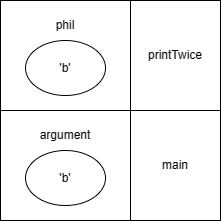
\includegraphics[height=6cm]{images/stack.png}
    \caption{Stack diagram from when printTwice is called}
    \label{fig:stack}
\end{figure}
%
Whenever a function is called, it creates a new {\bf instance}
of that function.  Each instance of a function contains the
parameters and local variables for that function.  In the
diagram an instance of a function is represented by a box
with the name of the function on the outside and the variables
and parameters inside.

In the example, {\tt main} has one local variable, {\tt argument}, and
no parameters.  {\tt printTwice} has no local variables and one
parameter, named {\tt phil}.

\section {Functions with multiple parameters}
\index{parameter!multiple}
\index{function!multiple parameter}
\index{class!Time}

The syntax for declaring and invoking functions with multiple
parameters is a common source of errors.  First, remember
that you have to declare the type of every parameter.  For
example

\begin{verbatim}
  void printTime (int hour, int minute) {
    cout << hour;
    cout << ":";
    cout << minute;
  }
\end{verbatim}
%
It might be tempting to write {\tt (int hour, minute)}, but
that format is only legal for variable declarations, not
for parameters.

Another common source of confusion is that you do not have
to declare the types of arguments.  The following is wrong!

\begin{verbatim}
    int hour = 11;
    int minute = 59;
    printTime (int hour, int minute);   // WRONG!
\end{verbatim}
%
In this case, the compiler can tell the type of {\tt hour}
and {\tt minute} by looking at their declarations.  It is
unnecessary and illegal to include the type when you pass them
as arguments.  The correct
syntax is {\tt printTime (hour, minute)}.

\label{printparity}
Do you remember the if/else code we did in the last chapter to check if something was even or odd? If you think you might want to check the parity
(evenness or oddness) of numbers often, you might want to
``wrap'' this code up in a function, as follows:

\begin{lstlisting}

void printParity (int x) {
  if (x%2 == 0) {
    std::cout << "x is even" << std::endl;
  } else {
    std::cout << "x is odd" << std::endl;
  }
}
\end{lstlisting}
%
Now you have a function named {\tt printParity} that will display
an appropriate message for any integer you care to provide. It is perfectly acceptable to have an if statement in a function.
In {\tt main} you would call this function as follows:

\begin{verbatim}
    printParity (17);
\end{verbatim}
%
Always remember that when you {\em call} a function, you do
not have to declare the types of the arguments you provide.
C++ can figure out what type they are.  You should resist the
temptation to write things like:

\begin{verbatim}
  int number = 17;
  printParity (int number);         // WRONG!!!
\end{verbatim}
\section {Functions with results}
\index{fruitful function}
\index{function!fruitful}

You might have noticed by now that some of the functions we are using,
like the math functions, yield results.  Other functions,
like {\tt newLine}, perform an action but
don't return a value.  That raises some questions:

\begin{itemize}

\item What happens if you call a function and you don't
do anything with the result (i.e. you don't assign it to
a variable or use it as part of a larger expression)?

\item What happens if you use a function without a result as part
of an expression, like {\tt newLine() + 7}?

\item Can we write functions that yield results, or are we
stuck with things like {\tt newLine} and {\tt printTwice}?

\end{itemize}

The answer to the third question is ``yes, you can write functions that
return values,'' and we'll do it in Chapter~\ref{fruitful functions}.  I will
leave it up to you to answer the other two questions by trying them
out.  Any time you have a question about what is legal or
illegal in C++, a good way to find out is to ask the compiler.

\section{The {\tt return} statement}
\index{return}
\index{statement!return}

The {\tt return} statement allows you to terminate the execution
of a function before you reach the end.  One reason to use it
is if you detect an error condition:

\begin{verbatim}
#include <cmath>

void printLogarithm (double x) {
  if (x <= 0.0) {
    cout << "Positive numbers only, please." << endl;
    return;
  }

  double result = log (x);
  cout << "The log of x is " << result;
}
\end{verbatim}
%
This defines a function named {\tt printLogarithm} that takes
a {\tt double} named {\tt x} as a parameter.  The first thing
it does is check whether {\tt x} is less than or equal to
zero, in which case it displays an error message and then uses
{\tt return} to exit the function.  The flow of execution
immediately returns to the caller and the remaining lines of
the function are not executed.

I used a floating-point value on the right side of the condition
because there is a floating-point variable on the left.

Remember that any time you want to use one a function from the math
library, you have to include the header file {\tt math.h}.

\section{Recursion}
\label{recursion}
\index{recursion}

I mentioned in the last chapter that it is legal for one function to
call another, and we have seen several examples of that.  I neglected
to mention that it is also legal for a function to call itself.  It
may not be obvious why that is a good thing, but it turns out to be
one of the most magical and interesting things a program can do.

For example, look at the following function:

\begin{verbatim}
void countdown (int n) {
  if (n == 0) {
    cout << "Blastoff!" << endl;
  } else {
    cout << n << endl;
    countdown (n-1);
  }
}
\end{verbatim}
%
The name of the function is {\tt countdown} and it takes a single
integer as a parameter.  If the parameter is zero, it outputs
the word ``Blastoff.''  Otherwise, it outputs the parameter and
then calls a function named {\tt countdown}---itself---passing
{\tt n-1} as an argument.

What happens if we call this function like this:

\begin{verbatim}
#include <iostream>
#include <cmath>
using namespace std;
void printLogarithm (double x) {
  if (x <= 0.0) {
    cout << "Positive numbers only, please." << endl;
    return;
  }

  double result = log (x);
  cout << "The log of x is " << result;
}

void countdown (int n) {
  if (n == 0) {
    cout << "Blastoff!" << endl;
  } else {
    cout << n << endl;
    countdown (n-1);
  }
}

int main ()
{
  countdown (3);
  return 0;
}
\end{verbatim}
%
The execution of {\tt countdown} begins with {\tt n=3}, and
since {\tt n} is not zero, it outputs the value 3, and then
calls itself...

\begin{quote}
The execution of {\tt countdown} begins with {\tt n=2}, and
since {\tt n} is not zero, it outputs the value 2, and then
calls itself...

\begin{quote}
The execution of {\tt countdown} begins with {\tt n=1}, and
since {\tt n} is not zero, it outputs the value 1, and then
calls itself...

\begin{quote}
The execution of {\tt countdown} begins with {\tt n=0}, and
since {\tt n} is zero, it outputs the word ``Blastoff!''
and then returns.
\end{quote}

The countdown that got {\tt n=1} returns.

\end{quote}

The countdown that got {\tt n=2} returns.

\end{quote}

The countdown that got {\tt n=3} returns.

\noindent And then you're back in {\tt main} (what a trip).  So the
total output looks like:

\begin{verbatim}
3
2
1
Blastoff!
\end{verbatim}
%
As a second example, let's look again at the functions
{\tt newLine} and {\tt threeLine}.

\begin{verbatim}
void newLine () {
  cout << endl;
}

void threeLine () {
  newLine ();  newLine ();  newLine ();
}
\end{verbatim}
%
Although these work, they would not be much help if I wanted
to output 2 newlines, or 106.  A better alternative would be

\begin{verbatim}
void nLines (int n) {
  if (n > 0) {
    cout << endl;
    nLines (n-1);
  }
}
\end{verbatim}
%
This program is similar to {\tt countdown}; as long as {\tt n} is
greater than zero, it outputs one newline, and then calls itself to
output {\tt n-1} additional newlines.  Thus, the total number of
newlines is {\tt 1 + (n-1)}, which usually comes out to roughly {\tt
n}.

\index{recursive}
\index{newline}

The process of a function calling itself is called {\bf recursion}, and
such functions are said to be {\bf recursive}.

\section {Infinite recursion}

In the examples in the previous section, notice that each time the
functions get called recursively, the argument gets smaller by one, so
eventually it gets to zero.  When the argument is zero, the function
returns immediately, {\em without making any recursive calls}.
This case---when the function completes without making a recursive
call---is called the {\bf base case}.

If a recursion never reaches a base case, it will go on making recursive
calls forever and the program will never terminate.  This is known as
{\bf infinite recursion}, and it is generally not considered a good
idea.

\index{recursion!infinite}
\index{infinite recursion}
\index{run-time error}

In most programming environments, a program with an infinite
recursion will not really run forever.  Eventually, something
will break and the program will report an error.  This is the
first example we have seen of a run-time error (an error that
does not appear until you run the program).

You should write a small program that recurses forever and run
it to see what happens.

\section {Stack diagrams for recursive functions}
\index{stack}
\index{diagram!state}
\index{diagram!stack}

In a previous section we used a stack diagram to represent the
state of a program during a function call.  The same kind
of diagram can make it easier to interpret a recursive function.

Remember that every time a function gets called it creates
a new instance that contains
the function's local variables and parameters.

This figure shows a stack diagram for countdown, called
with {\tt n = 3}:

\vspace{0.1in}
\centerline{\epsfig{figure=oldimages/stack2.eps}}
\vspace{0.1in}
%
There is one instance of {\tt main} and four instances of
{\tt countdown}, each with a different value for the parameter
{\tt n}.  The bottom of the stack, {\tt countdown} with {\tt n=0}
is the base case.  It does not make a recursive call, so there
are no more instances of {\tt countdown}.

The instance of {\tt main} is empty because {\tt main} does not
have any parameters or local variables.  As an exercise, draw a
stack diagram for {\tt nLines}, invoked with the parameter {\tt n=4}.



\section{Glossary}

\begin{description}

\item[initialization:]  A statement that declares a new variable
and assigns a value to it at the same time.

\item[function:]  A named sequence of statements that performs some
useful function.  Functions may or may not take parameters, and may
or may not produce a result.

\item[parameter:]  A piece of information you provide
in order to call a function.  Parameters are like variables in
the sense that they contain values and have types.

\item[argument:]  A value that you provide when you call a
function.  This value must have the same type as the corresponding
parameter.

\item[call:]  Cause a function to be executed.

\item[recursion:]  The process of calling the same function you
are currently executing.

\item[infinite recursion:]  A function that calls itself
recursively without every reaching the base case.  Eventually
an infinite recursion will cause a run-time error.

\index{function}
\index{parameter}
\index{argument}
\index{call}
\index{initialization}
\index{recursion}
\index{recursion!infinite}
\index{infinite recursion}

\end{description}

